\begin{figure}[H]
\centering
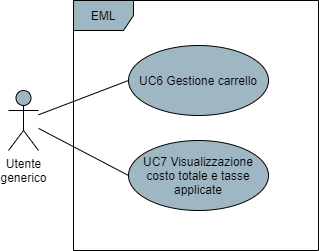
\includegraphics[scale=0.6]{res/UseCase/Immagini/CarrelloGenerale}
\caption{Schema generale: modulo del carrello}
\end{figure}

\subsubsection{UC6 - Gestione prodotti carrello}
\begin{itemize}
\item \textbf{Attori primari}: utente generico;
\item \textbf{Descrizione}: per tutti gli utenti è disponibile una pagina del carrello in cui è possibile visualizzare e gestire i prodotti inseriti al suo interno. È successivamente possibile acquistare i prodotti presenti nel carrello;
\item \textbf{Scenario Principale}: un utente generico si trova all'interno della pagina del carrello ed ha a disposizione queste funzionalità per la gestione dei prodotti al suo interno:
\begin{itemize}
\item visualizzazione prodotti nel carrello [\textbf{UC6.1}];
\item rimozione prodotto dal carrello [\textbf{UC6.2}];
\item modifica quantità di un prodotto nel carrello [\textbf{UC6.3}];
\end{itemize}
\item \textbf{Precondizione}: l'utente generico si trova nel sito ed ha a disposizione la pagina del carrello;
\item \textbf{Postcondizione}: l'utente ha a disposizione varie funzionalità per gestire i prodotti all'interno del carrello.
\end{itemize}

\begin{figure}[H]
\centering
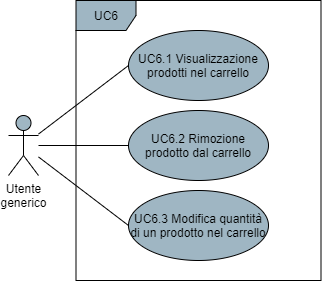
\includegraphics[scale=0.6]{res/UseCase/Immagini/GestioneCarrello}
\caption{Diagramma UML\ped{G} per UC6 - Gestione prodotti carrello}
\end{figure}

\subsubsection{UC6.1 - Visualizzazione prodotti nel carrello}
\begin{itemize}
\item \textbf{Attori primari}: utente generico;
\item \textbf{Descrizione}: l'utente generico visualizza una lista di prodotti precedentemente inseriti nel carrello;
\item \textbf{Scenario Principale}: l'utente generico si trova nella pagina del carrello e visualizza i seguenti dati per ogni prodotto inserito nel carrello:
\begin{itemize}
\item nome del prodotto;
\item immagine del prodotto;
\item quantità presente nel carrello;
\item costo del prodotto.
\end{itemize}
\item \textbf{Precondizione}: l'utente generico si trova nella pagina del carrello;
\item \textbf{Postcondizione}: viene visualizzata la lista di prodotti presenti nel carrello.
\end{itemize}

\subsubsection{UC6.2 - Rimozione prodotto nel carrello}
\begin{itemize}
\item \textbf{Attori primari}: utente generico;
\item \textbf{Descrizione}: l'utente generico può rimuovere un prodotto precedentemente inserito nel carrello;
\item \textbf{Scenario Principale}: l'utente generico si trova nella pagina del carrello e clicca un tasto dedicato per rimuovere un prodotto dal carrello;
\item \textbf{Precondizione}: l'utente generico si trova nella pagina del carrello e ha almeno un prodotto al suo interno;
\item \textbf{Postcondizione}: il prodotto rimosso non è più presente nel carrello.
\end{itemize}

\subsubsection{UC6.3 - Modifica quantità di un prodotto nel carrello}
\begin{itemize}
\item \textbf{Attori primari}: utente generico;
\item \textbf{Descrizione}: l'utente generico può modificare la quantità di un prodotto precedentemente inserito nel carrello;
\item \textbf{Scenario Principale}: l'utente generico si trova nella pagina del carrello e clicca dei tasti dedicati per modificare la quantità di un prodotto, incrementandola o decrementandola;
\item \textbf{Precondizione}: l'utente generico si trova nella pagina del carrello e ha almeno un prodotto al suo interno;
\item \textbf{Postcondizione}: viene modificata la quantità di un prodotto del carrello in base all'intento dell'utente.
\end{itemize}

\subsubsection{UC7 Visualizzazione costo totale e tasse applicate}
\begin{itemize}
\item \textbf{Attori primari}: utente generico;
\item \textbf{Descrizione}: l'utente generico visualizza le tasse applicate e il costo totale dei prodotti nel suo carrello;
\item \textbf{Scenario Principale}: l'utente generico si trova nella pagina del carrello e visualizza il costo totale e le tasse applicate ad essi;
\item \textbf{Precondizione}: l'utente generico si trova nella pagina del carrello e ha almeno un prodotto al suo interno;
\item \textbf{Postcondizione}: viene visualizzato il costo totale dei prodotti del carrello e le tasse applicate.
\end{itemize}




